\chapter{Proposed solution and Implementation} 

\section{Chosen solution}

The following decisions and use cases were considered:

\begin{itemize}
 \item The subjects of the irrigation are indoor plants.
 \item The water source is a bucket.
 \item The controller is implemented using an Arduino Mega microcontroller.
 \item The controller must be calibrated for each plant: one must measure the moisture in the soil in both extreme cases.
 \item The user can configure the controller parameters: e.g. the threshold moisture level.
 \item The configuration interface is a REST web server, hosted on a ESP8266 Wi-Fi shield with the AT firmware.
\end{itemize}

The following features were also included in the system:

\begin{itemize}
 \item Persisting the configuration parameters in EEPROM
 \item Allowing the user to set the extreme values by pressing buttons
 \item Displaying the moisture percentage or eventual errors on a seven segment display
\end{itemize}






\section{Algorithms}

\subsection{Controlling the moisture level}
\label{sec:control_fsm}

\begin{figure}[ht]
    \centering
    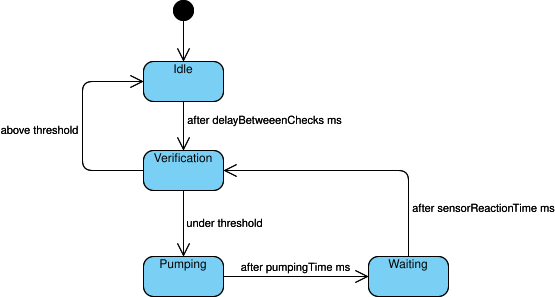
\includegraphics[width=\linewidth]{img/Irrigation station controller state diagram.png}
    \caption{The state diagram of the moisture level controller}
    \label{fig:controller_state_diagram}
\end{figure}

The controller can be considered as a state machine (figure \ref{fig:controller_state_diagram})  which changes states based on the sensor readings and on the timing parameters configured by the user.

In the \textbf{idle state} the controller waits. The \verb|delayBetweenChecks| parameter specifies the duration the controller stays in this state. After that it moves to the verification state.

In the \textbf{verification state} the sensor value is read, converted to percentage based on the saved extreme values, and  finally, it is compared with the threshold value. In case it is lower, the pumping state follows, in the other case the controller moves back to the idle state.

In the \textbf{pumping state} the pump is enabled and the water flows from the tank to the plant. The duration of pumping is given by the \verb|pumpingTime| parameter. After that it moves to the waiting state.

In the \textbf{waiting state} the controller waits for the sensor to react to the water flowing from the pump. The duration is given by the \verb|sensorReactionTime| parameter. Then it moves to the verification state.

\subsection{Parsing HTTP requests byte-by-byte}
\label{sec:http_fsm}

From the HTTP requests only the request type and the endpoint are considered, the rest is ignored. Therefore another state machine was used which reads the characters from the Wi-Fi module, and saves only these two strings into separate variables. The state transitions happen on reading the \verb|' '| character.





\section{Implementation}

\section{Hardware} 

\begin{figure}[ht]
    \centering
    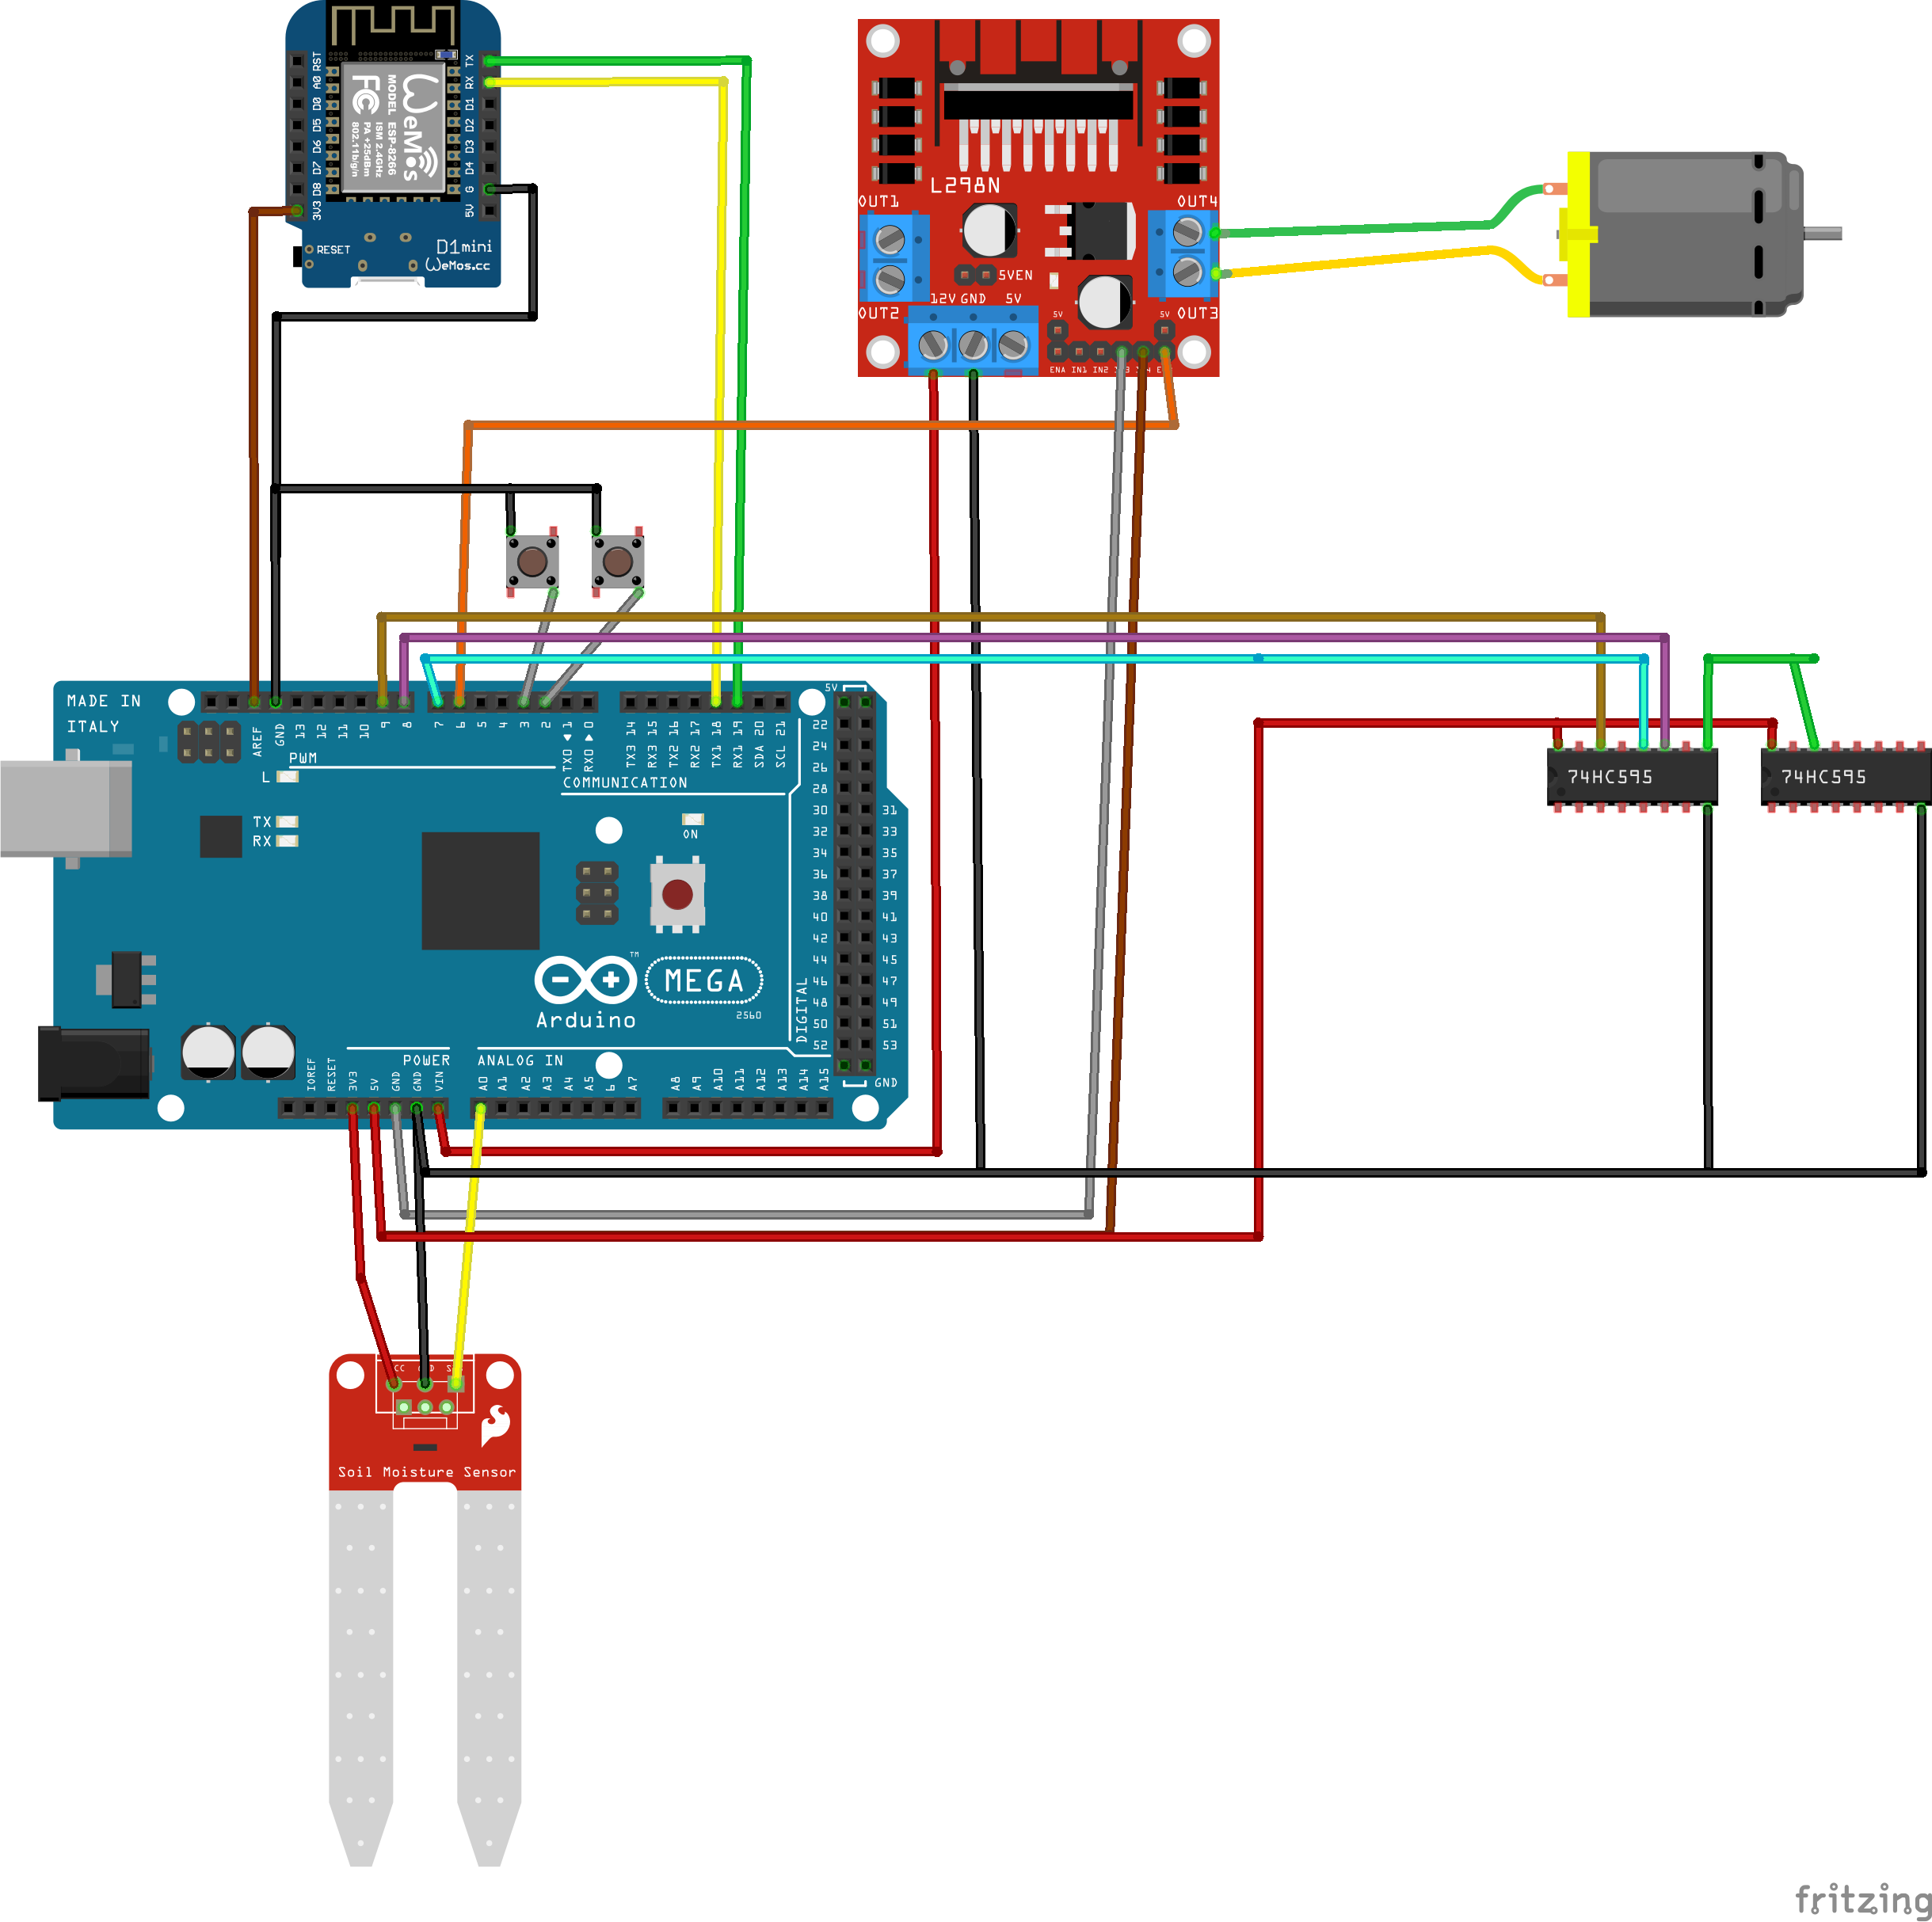
\includegraphics[width=\linewidth]{img/IrrigationStationHardware.png}
    \caption{The overview of the hardware components and their interconnections}
    \label{fig:hardware_diagram}
\end{figure}

\begin{figure}[ht]
    \centering
    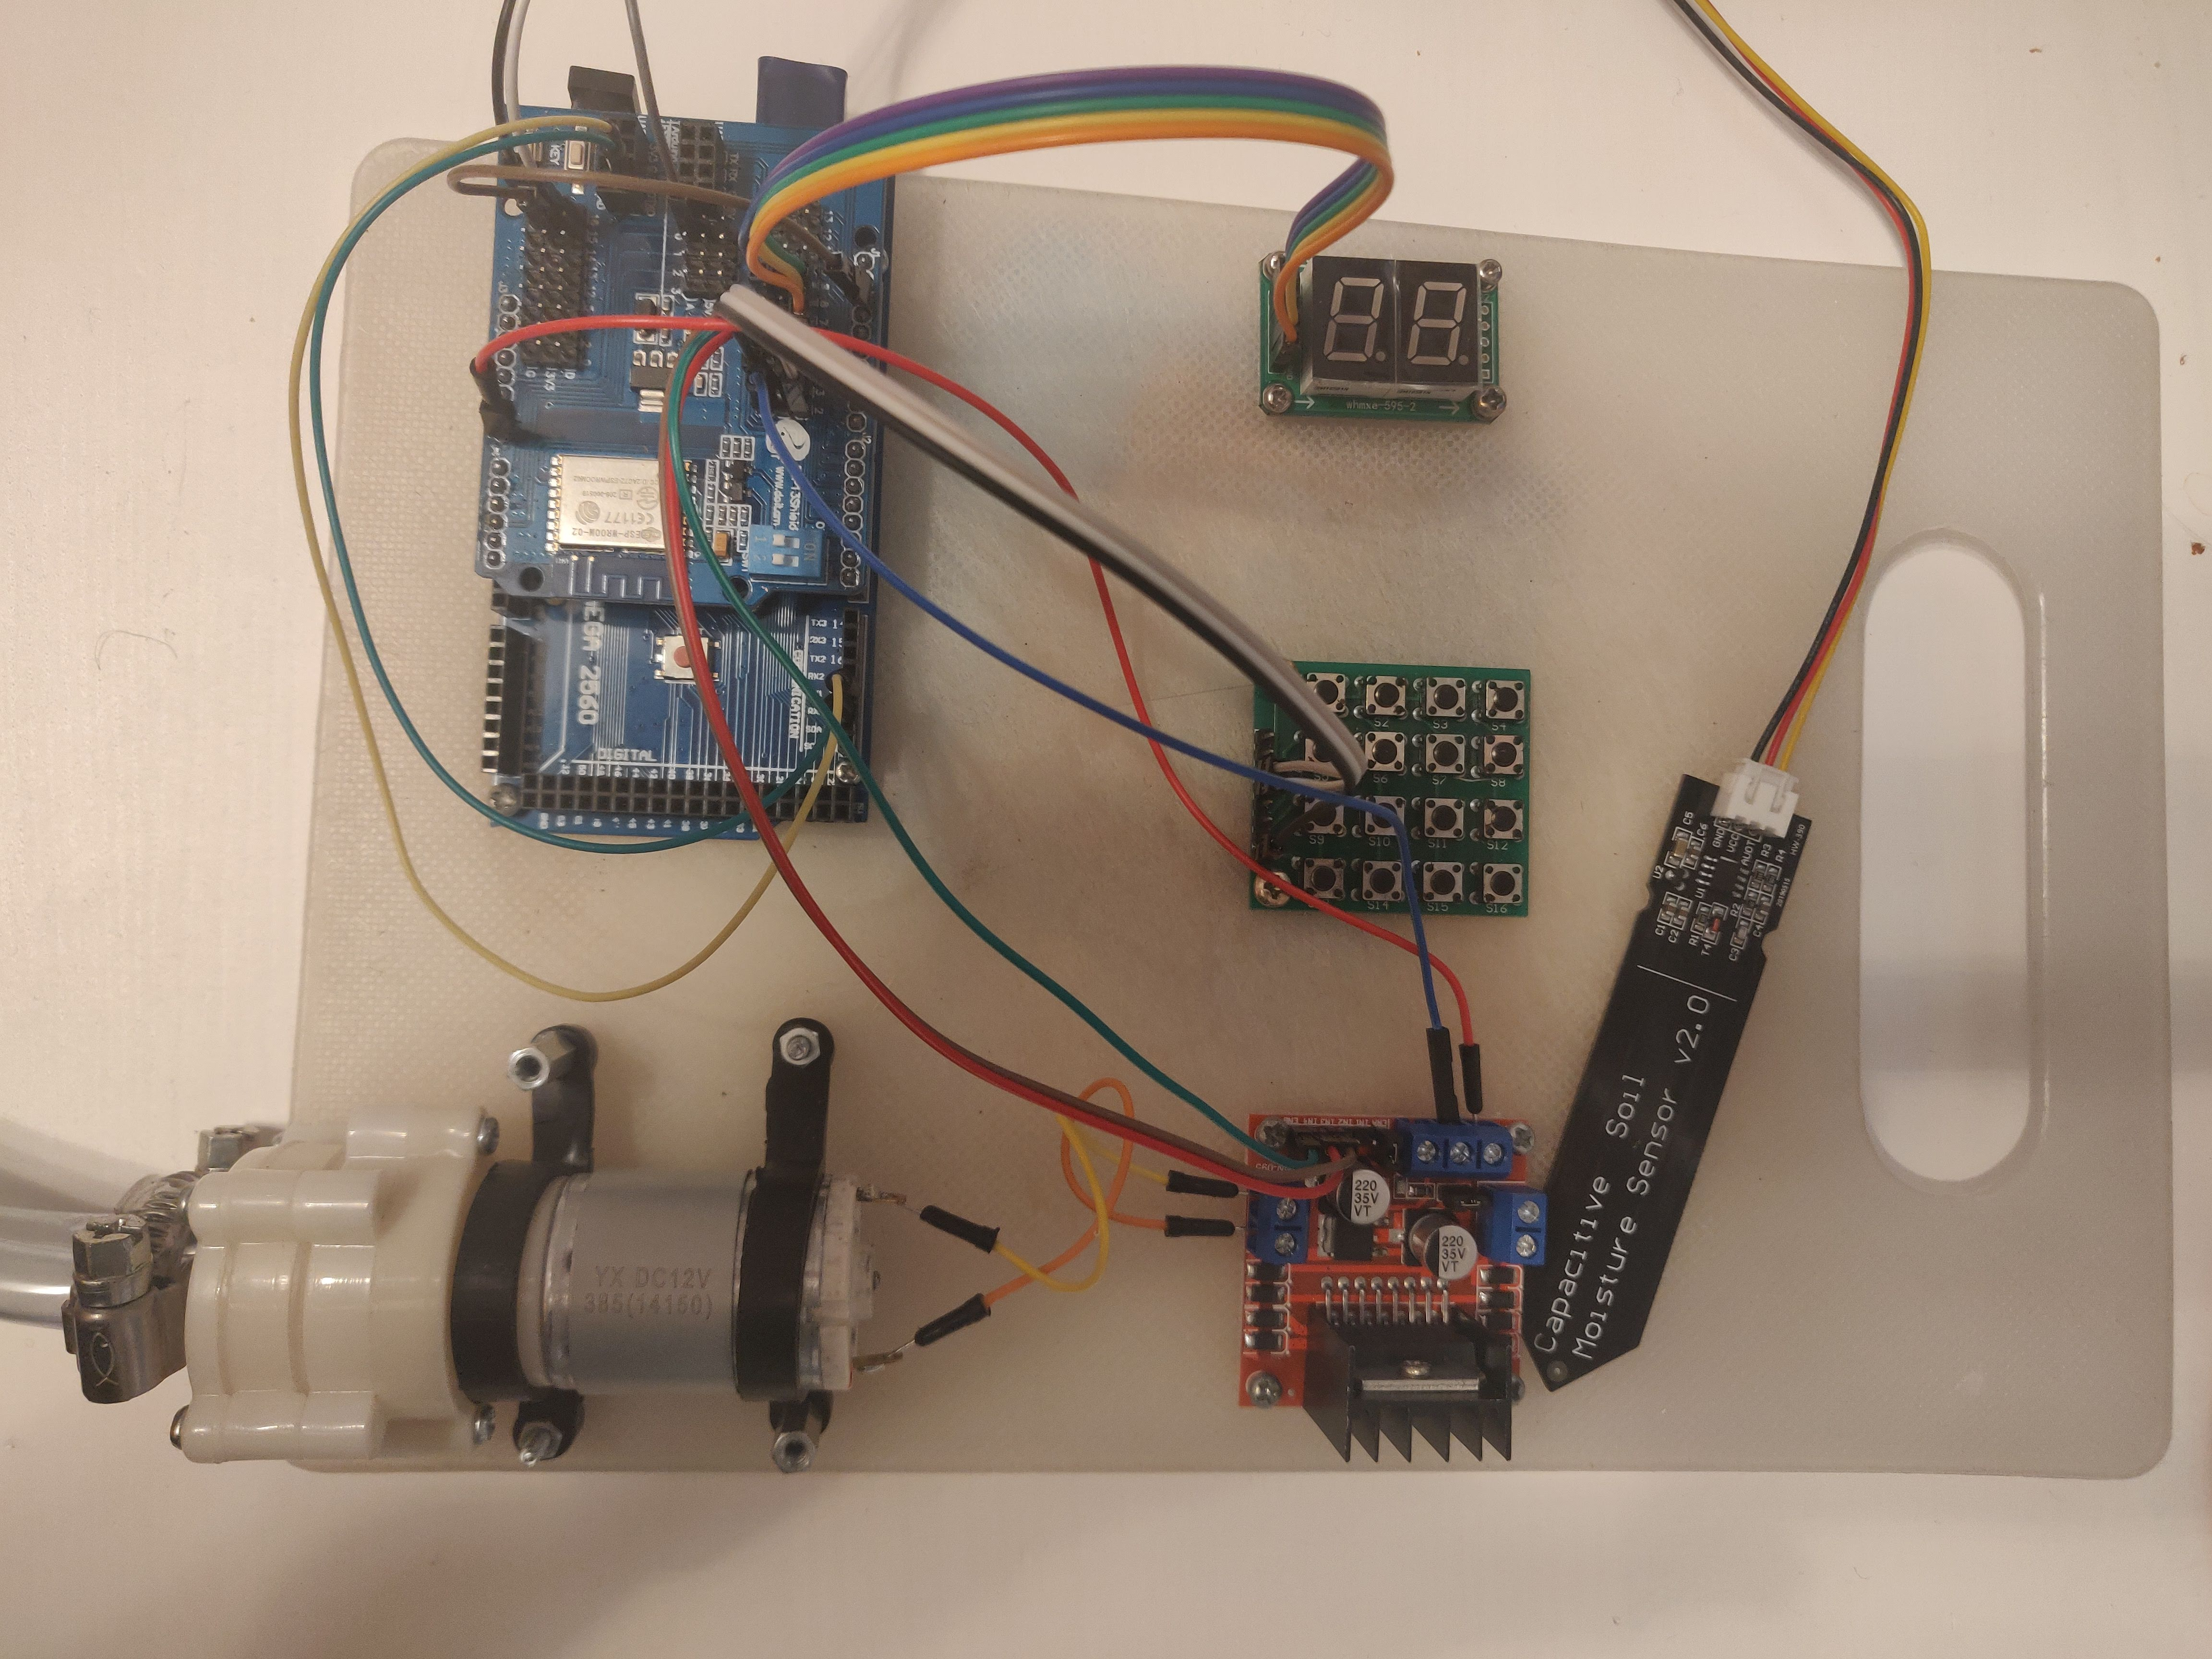
\includegraphics[width=\linewidth]{img/components.jpg}
    \caption{Picture of the components and their interconnection}
    \label{fig:components}
\end{figure}

Figure \ref{fig:hardware_diagram} shows the components used in the project. Figure \ref{fig:components} shows the real circuit.

An \textbf{Arduino Mega 2560} was used for controlling the moisture level. The program is uploaded on it. It receives 12V power through the DC jack.

For wireless communication a \textbf{DoIt ESP-13 Wi-Fi shield} was used. The AT firmware was uploaded to its ESP8266 chip. On figure \ref{fig:hardware_diagram} a different ESP component appears, because of the limitation in the design program. The voltage level shifters and regulators were hidden from the diagram because it is part of the shield. Therefore the TX and RX is directly connected to RX and TX of Arduino and the 5V port is unconnected on the image.

A 12V \textbf{water pump} was used for supplying water to the plants. This component works like a DC motor. Therefore it is represented as a motor on the image.

The pump needs a motor driver. Thus the \textbf{L298n motor driver} was added to the circuit. Its 12V power source is the external input voltage of the Arduino (VIN). The direction of the motor is hardwired, to pump only in one direction. The enable pin however is connected to the D6 pin of the Arduino board. Through this the microcontroller can turn on/off the pump or set its speed by using PWM.

A \textbf{capacitive moisture level sensor} was connected to the A0 pin of the board. It's supply voltage is 3.3V. The component differs from the one on the image because its capacitive, it is a single rod, and it can be directly connected to the board.

Two \textbf{buttons} are connected to the interrupt pins of the board. They are used for setting the extreme sensor values. When they are pressed, the program reads the sensor value and updates the current parameter with it.


Two \textbf{seven segment displays} are connected to the circuit. Their anodes are connected to '1' so the program must specify only their cathodes. The module containing the display manages this by using two 74HC595 shift registers. Therefore the only wires that are connected to the board are the: SDI, SCLK, LOAD. Thus the internal implementation of the module is not present on the diagram.

\section{Software}

The main program is defined in \verb|controller.ino|. In the \verb|setup()| function it displays the ``SE'' characters on the seven segment display, and calls the setup functions of each module. It has a \textbf{suspend flag}. When it is set, the loop function immediately returns, thus the program not executing anything anymore.

To achieve parallelism, the ``Timer.h'' library was used, which calls the given methods after the specified duration, by using the \verb|millis()| function. This library was used for handling the timings of the moisture controller presented in section \ref{sec:control_fsm}. Its implementation can be found in the \verb|processing.ino| file.

The \verb|config.h| file contains the constants of the program and also the application parameters. The \verb|Settings| data structure contains those parameters that can be modified by the user. The settings are read from the EEPROM and updated every time the field values change. The \verb|settings.ino| file implements the saving, loading and printing of this structure.

The \verb|moisture_sensor.ino| file handles the operations on the capacitive  soil moisture level sensor. It provides functions for reading the sensor value, handles the conversion  between the sensor value, the voltage value and the percentage. It also provides two functions for updating the two extreme sensor values.

The \verb|interrupts.ino| file configures the two buttons to trigger the interrupts. It also implements the interrupt service routines of them. These functions need to apply debouncing first, then they call the previously mentioned functions for updating the extreme values.

The \verb|pump.ino| file contains the functions for handling hte pump operations.

The \verb|display.ino| file handles the printing of characters and numbers to the seven segment displays. It contains a lookup table for all printable characters.

The \verb|error.h| contains an enum with all the system errors and their string representations. These are the errors that can be shown on the seven segment displays. The `\verb|error.ino| file contains the function which displays an error on the display, then it sets the \textit{suspend flag}.

The ``WiFiEsp.h'' library was used for the serial communication with the ESP8266 module, using the AT commands. In \verb|wifi.ino| functions are implemented which handle the setup of the module, the printing of the Wi-Fi data and the receiving of the clients. The latter function is called in the \verb|loop()| method of the main program. When the ESP module opens a socket this function receives a client object and reads the HTTP request character-by-character. The finite-state-machine described in \ref{sec:http_fsm} was used for parsing the input and saving the HTTP request type and the endpoint.

The requests are handled by the functions of the \verb|endpoints.ino| file. The \verb|handleRequest()| function receives a client, the request type and the endpoint, and routes it to the other methods. These function each implement and endpoint individually. The list of the endpoints and the corresponding functions can be seen in table \ref{tab:enpoints}. To send an receive JSON messages, the ``ArduinoJson.h'' library was used.

In case of an unparsable input, an inexisting endpoint, an unavailable request type or invalid input the corresponding HTTP responses are returned: BAD REQUEST, NOT FOUND, METHOD NOT ALLOWED, UNPROCESSABLE ENTITY. If the functions are executed correctly, the OK response is returned.

The \verb|http.h| header contains the HTTP status codes which are used in the program with their string representation. The \verb|http.ino| file implements methods for sending HTTP responses

The \verb|util.h| file contains the utility functions, such as \verb|average()|, which calculates the average of returned values when calling a function repeated times. This is used for reading the sensor data.

\subsubsection{Debugging}

For debugging, the program prints values to its main serial port, which is connected to the USB port. When the program starts, it prints the saved configuration values and also other data related to the wifi connection, such as its local ip address.


\begin{table}[ht]
 \centering
 \begin{tabular}{| l | c | l | p{0.55\linewidth} |} 
    \hline
    Function & Request & Endpoint & Action \\ [0.5ex] 
    \hline\hline
    getRoot & GET & / & Show all endpoints\\ 
    \hline
    getSensor & GET & /sensor & Show the parameters related to the sensor readings:
    \begin{itemize}
     \item The range of valid values: min and max
     \item The extreme values: dry and wet
     \item The threshold percentage
    \end{itemize}\\ 
    \hline
    updateSensor & PATCH & /sensor & Update the parameters. Each specified input value is validated. The HTTP response tells if the execution was a success\\ 
    \hline
    getSensor & GET & /moisture & Show the current moisture value in multiple formats:
    \begin{itemize}
     \item Raw sensor reading
     \item Voltage 
     \item Percentage
    \end{itemize}\\ 
    \hline
    getTiming & GET & /timing & Show the parameters related to the timing:
    \begin{itemize}
     \item sensorReactionTime - parameter of the controller
     \item pumpingTime - parameter of the controller
     \item delayBetweenChecks - parameter of the controller
     \item displayRefreshPeriod - specifies the waiting period after updating the percentage on the 7-segment display
    \end{itemize}\\ 
    \hline
    updateTiming & PATCH & /timing & Update the parameters. Each specified input value is validated. The HTTP response tells if the execution was a success\\ [1ex] 
    \hline
 \end{tabular}
 \caption{The endpoints of the web server and the corresponding functions which implement them}
 \label{tab:enpoints}
\end{table}







